\documentclass[a4paper]{article}
\renewcommand{\familydefault}{\sfdefault}
\usepackage[english]{babel}
\usepackage[utf8x]{inputenc}
\usepackage{amsmath}
\usepackage{graphicx}

\title{ERCore Technical Description}
\author{MetOcean Solutions Ltd.}

\begin{document}
\maketitle

\section{Introduction}

ERCore is a Lagrangian particle tracking model for simulating the dispersion and fate of material in the oceanic or atmospheric environment.
It solves equations describing the movement and modification of discrete particles in response to the environment. The ambient flow of water or wind advects the particles with (usually) spatially and temporally varying fields.  
Turbulent diffusion is included with a random walk approach and the presence of a boundary such as a shoreline or the air-sea interface can be specified.
A simulated particle can represent any material with additional physical, chemical or biological processes added as required to simulate active modifications that may occur as it moves within the water or air.
Examples of active particles include sediment, oil, plankton and even persons lost at sea.

This document describes the mathematical and numerical formulation of the model.
Also included are descriptions of the various extensions that can be applied to the particles to allow them to simulate different materials.


\section{Numerical formulation}
\subsection{Equations of motion}
\begin{figure}
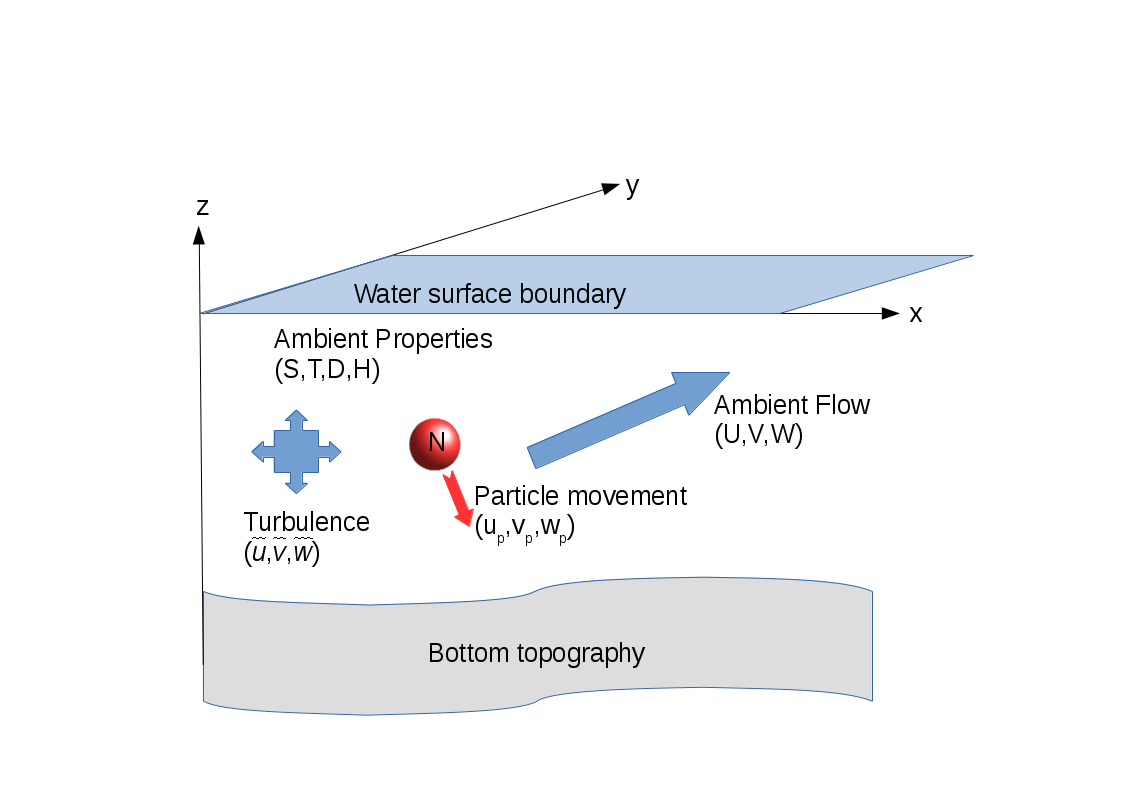
\includegraphics[width=\textwidth]{model.png}
\caption{Schematic of physical processes acting on a particle in the model.}
\end{figure}

The coordinate system is defined with $z$ positive upwards. The nominal 0 level for $z$ is Mean Sea Level, however any consistent vertical reference can be used.
The change position $x,y,z$ of a particle at time $t$ is governed by:\begin{align}
\frac{dx}{dt} = U(x,y,z,t)+\tilde{u}+u_p \\
\frac{dy}{dt} = V(x,y,z,t)+\tilde{v}+v_p \\ 
\frac{dz}{dt} = W(x,y,z,t)+\tilde{w}+w_p 
\end{align}
where $U,V,W$ is the ambient flow and $\tilde{u},\tilde{v},\tilde{w}$ are a turbulent flow component. $u_p,v_p,w_p$ are any additional motions that are properties of the particle's interaction with the surrounding water or air such as sinking, floating, drifting or swimming.

Each particle has a weighting and age attribute attached to it. The weight value can represent any measure of quantity depending on the application, for example mass, volume of number.
The generic equation describing the rate of change of weighting, $N$ is:
\begin{equation}\frac{dN}{dt}=f(P,U,V,W,S,T,D,H)\end{equation}
where $P$ are properties of the particle itself and $S,T,D,H$ are salinity, temperature, density and humidity of water or air.
Note that for a given process and medium only some of the ambient properties will be relevant. The age is a simple measure of time since a particle was released.
Any number of other attributes can also be attached to a particle which describe its physical, chemical or biological state.

\subsection{Turbulent diffusion}
The turbulent component of the velocity is given by:
\begin{align}
\int_{t}^{t+\Delta t} \tilde{u} dt = \sqrt{6K_h \Delta t} H(-1,1) \\
\int_{t}^{t+\Delta t} \tilde{v} dt = \sqrt{6K_h \Delta t} H(-1,1) \\
\int_{t}^{t+\Delta t} \tilde{w} dt = \sqrt{6K_v \Delta t} H(-1,1)
\end{align}
where $K_h$ and $K_v$ are horizontal and vertical eddy diffusion coefficients and $H$ is a number sampled from a uniform distribution bewteen $-1$ and $1$.
The eddy diffusion coefficients can be provided as known values, either constant or as a spatially (and temporally) varying field.

\subsection{Coordinate system}
The model solves all equations in standard SI units.
However the horizontal coordinates can also be configured as geographical longitude and latitude.
In this case a map factor is applied to any horizontal differences as:
\begin{align}
d\lambda = \frac{360dx}{C*cos{\theta}} \\
d\theta = \frac{360dy}{C}
\end{align}
where $\lambda$ and $phi$ are the longitude and latitude respectively. $C$ is the circumference of the earth.

\subsection{Numerical solution}
The equations of motion for each particle are integrated with a constant time step, $\Delta t$.
A Runge-Kutta scheme for the ambient flow component, with default order 4 (which can be reduced for computational speed by user configuration).
The turbulent and particle components of motion are added with a simple first order integration.

\subsection{Forcing fields}
The forcing fields $U,V,W$ are provided as input data which can be constant or as spatially and temporally varying fields.
For variable fields, the value at the particle position for a given time is determined by simple multilinear interpolation.
Any number of additional fields which can influence the particle can also be prescribed and are likewise interpolated to provide the local ambient conditions for the particle at each timestep.

\subsection{Boundaries}
Boundaries can be specified in 4 ways:
\begin{enumerate}
\item A shoreline vector
\item A spatially varying field (such as ocean depth) 
\item A constant level
\item A bounding box
\end{enumerate}
In each case an intersection algorithm is applied at each time-step to determine whether the particle crosses the boundary.
Firstly the particle motion vector for the time-step is calculated, then an intersect test is made between that vector and the boundaries.
Shorelines are defined as line segments, each of which is tested for intersection with the motion vector in the horizontal plane.
For variable boundaries such as the sea bottom, the z-coordinate at the start and end of the motion vector are first interpolated.
The straight line between these two z-coordinates is then used for the intersection test with the motion vector in the vertical plane;
the horizontal position of an intersect is then the fractional displacement in the horizontal direction.

If an intersection occurs, the particle is placed at the intersection point. 
The particles subsequent action at the following time-step depends on whether the boundary is sticky.
If the boundary is non-sticky the particle is free to move away from the boundary if its vector of motion carries it away.
In the case of a bounding box, the particle is removed from the simulation.

\begin{figure}
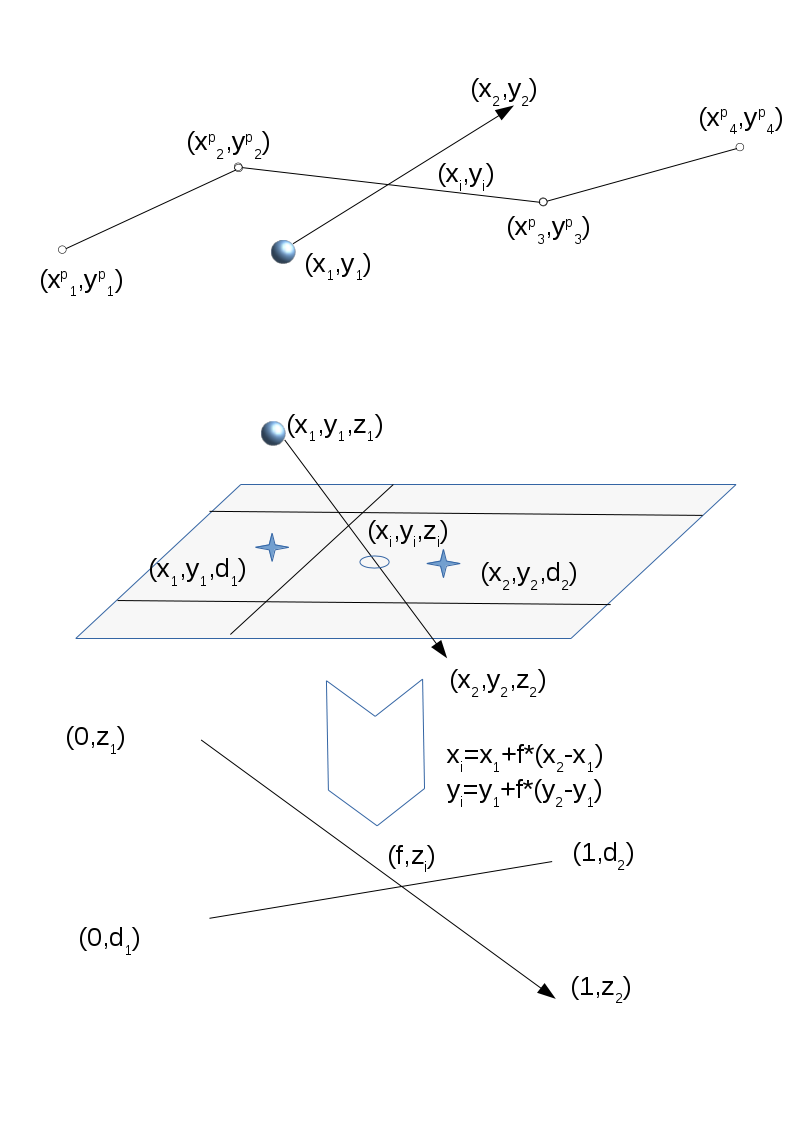
\includegraphics[width=\textwidth]{intersect.png}
\caption{Illustration of boundary crossing tests for shoreline (top) and variable surface (bottom).}
\end{figure}

\subsection{Particle release and tracking}
Particle releases are specified to be a particular location. In addition the following options are available:
\begin{enumerate}
\item Instantaneaous release of total material $M_{tot}$: All $n$ particles added at a given time.
\begin{equation} M=\frac{M_tot}{n} \end{equation}
\item Continuous release, with flux of material $F$: Particles are added continuously, at a rate of $n_{rel}$ every timestep $\Delta t_{rel}$.
\begin{equation}M=\frac{F}{\Delta t_{rel} n_{rel}}\end{equation} 
\item Staged release of total material $M_{tot}$ added over time.
\begin{equation}M=\frac{M_{tot}}{\Delta t_{rel}}\end{equation}
\end{enumerate}

Multiple releases can be specified and subsequently tracked.
A status code on each particle flags its state, for example whether it is releases and mobile, stuck to a boundary or has been removed.
The particle location and statuses are output at user specified intervals.

\section{Particle Processes}
\subsection{Biota}
Processes currently included that affect biota are:
\begin{enumerate}
\item Mortality in response to age, temperature or salinity
\item Spawning to become a subsequent life stage
\item Diurnal vertical migration
\end{enumerate}
Often, the weight property will represent number of organisms that each particle represents.

Mortality is modelled with a simple die-off rate:
\begin{equation}
\frac{dW}{dt}=-rW
\end{equation}
where $r$ is the mortality rate. The mortality rate, can either be specified as a constant value or as a function of temperature and/or salinity:
\begin{align}
r=\frac{T-T_L^{high}+T_{tol}}{T_{tol}} \in[0,1] \\
r=\frac{T_L^{low}+T_{tol}-T}{T_{tol}} \in[0,1]
\end{align}
where $T_L$ is the lethal temperature and $T_{tol}$ is a tolerance which describes the temperature range over which effects start to be felt.
Exactly analogous equations exist for salinity. When the particle weight drops below a prescribed number, the particle is removed from the simulation.

Diurnal vertical migration is determined by:
\begin{align}
w_p=w_m(t) \\
z \in [-z_{day},-z_{night}]
\end{align}
where $w_m$ is a vertical migration constant which is positive (up) after the sun sets, and negative down after sun rise.

Spawning occurs when biota either mature to their next life stage or release offspring.
In the first case the relevant class of the biota simply changes.
In the latter a new particle is created at the existing position, which its weight determined by a spawning ratio that describes the 

\subsection{Oil Spill}

\section{Configuration}



\end{document}
